\documentclass[12pt]{article}
\usepackage{amssymb,mathtools}
\usepackage[margin=1in]{geometry}
\usepackage{fancyhdr}
\usepackage{circuitikz}
\usepackage{graphicx}
\graphicspath{ {./Figures/} }
\usepackage{amsmath}
\usepackage{ragged2e}
\usepackage{subcaption} 
\usepackage{float}
\usepackage{cancel}
\usepackage{siunitx}
\pagestyle{fancy}
\usepackage[shortlabels]{enumitem}
\usepackage{mathtools}
\newcommand*{\permcomb}[4][0mu]{{{}^{#3}\mkern#1#2_{#4}}}
\newcommand*{\Comb}[2]{{}^{#1}C_{#2}}
\DeclarePairedDelimiter\ceil{\lceil}{\rceil}
\DeclarePairedDelimiter\floor{\lfloor}{\rfloor}
\setlength{\headheight}{15 pt}
\lhead{Georgy Antonov}
\chead{HW 5}
\rhead{Neural Dynamics}

\begin{document}\noindent


\noindent\textbf{Question 1. Simulation of a multi-compartment Hodgkin-Huxley model.}
\begin{enumerate}
    \item[1.1] The Hodgkin-Huxley model for an active neurite with input current $I_{e}(j, t)$ 
    for a single cylindrical compartment $j$ is given by equations 1-12.
    \begin{figure}[h!]
        \centering
        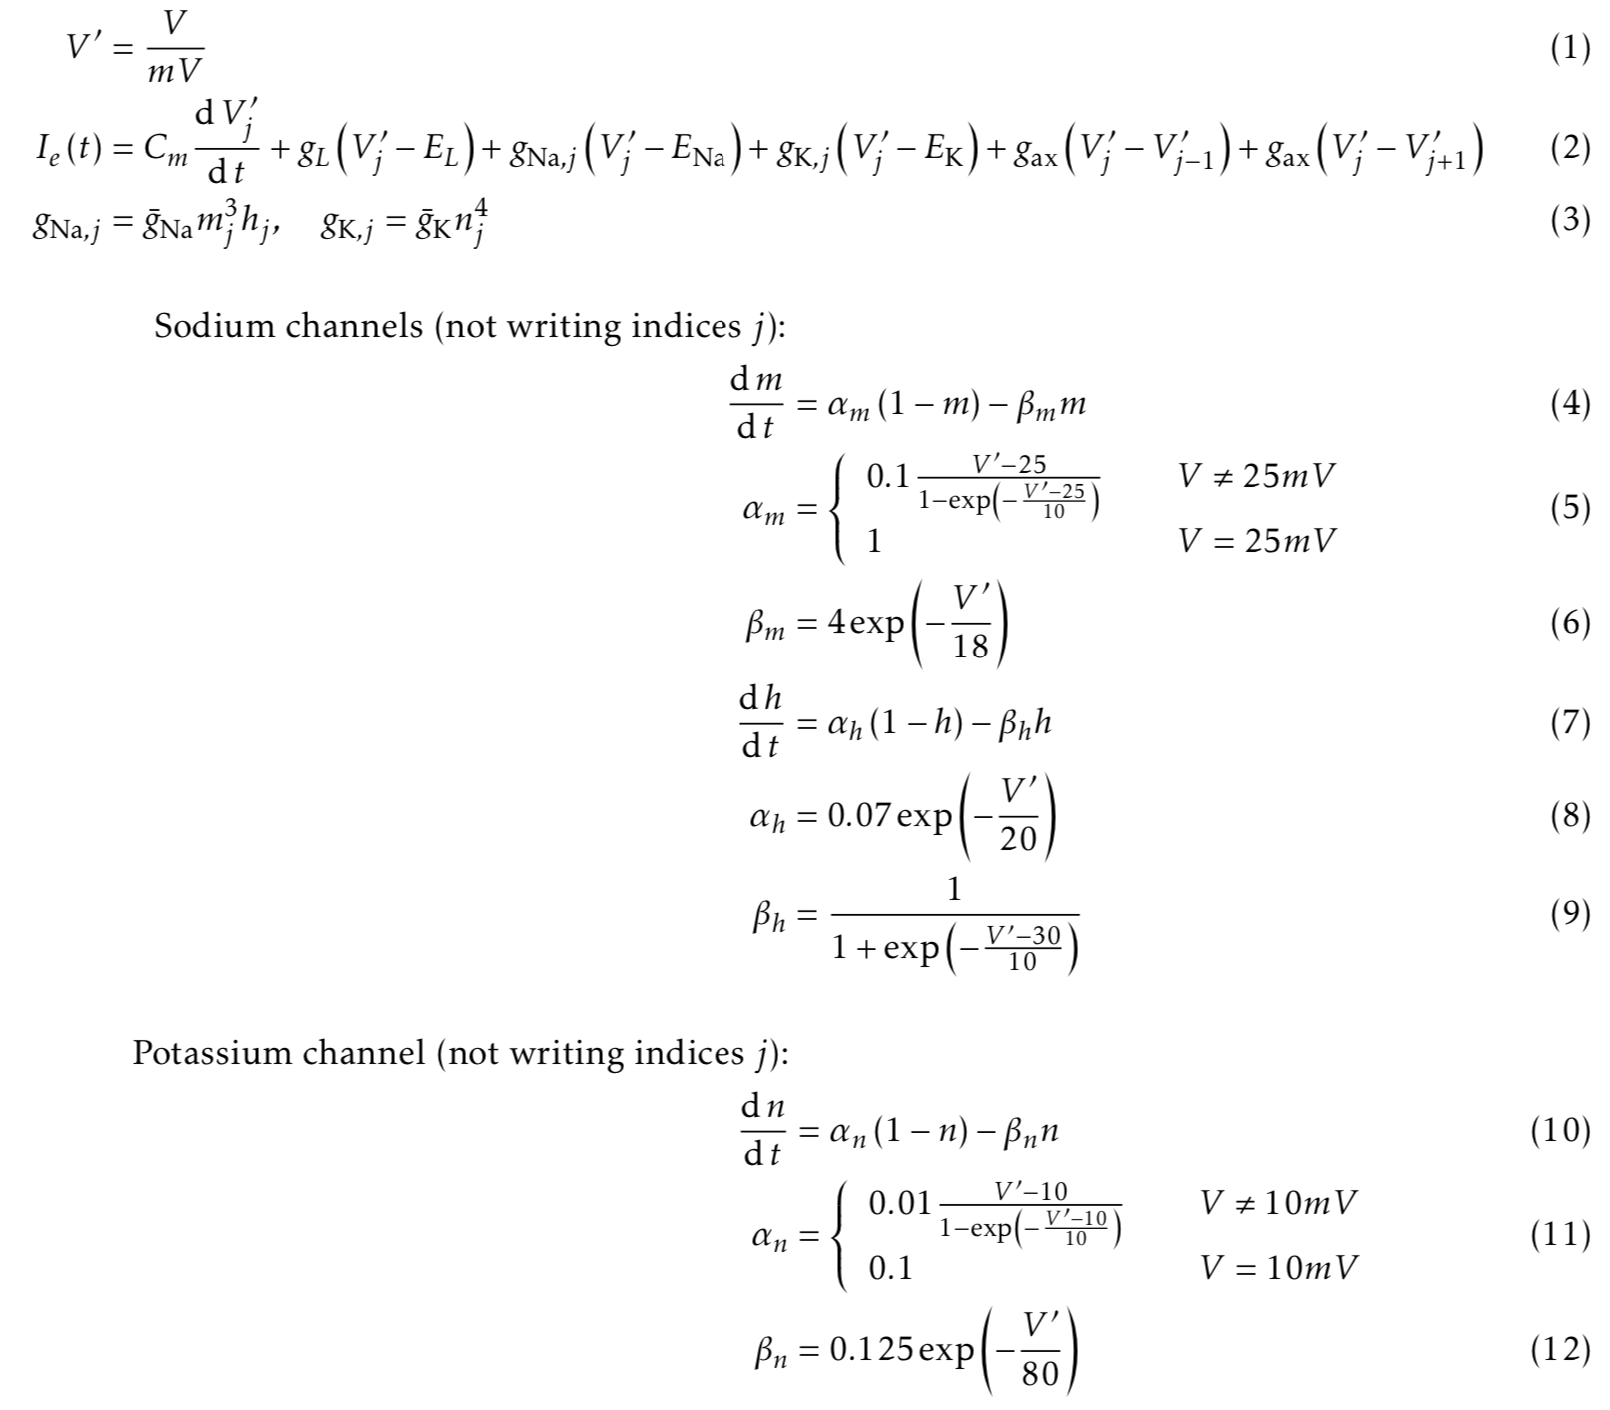
\includegraphics[width=1\textwidth]{Eqs.png}
    \end{figure}\\
    The electrical and geometrical properties are
    \begin{itemize}
        \item $C_{m} = 1 \, \mu \text{F}$, membrane capacitance
        \item $E_{Na}=115 \, \text{mV}$, sodium equilibrium potential
        \item $E_{K}=-12 \, \text{mV}$, potassium equilibrium potential
        \item $E_{L}=10.6 \, \text{mV}$, leak equilibrium potential
        \item $V(t=0)=0 \, \text{mV}$, initial (and equilibrium) membrane potential
        \item $\bar{g}_{Na}=120 \, \text{mS}$, maximum sodium channel conductance
        \item $\bar{g}_{K}=36 \, \text{mS}$, maximum potassium channel conductance
        \item $g_{L}=0.3 \, \text{mS}$, leak conductance
        \item $g_{ax}=0.5 \, \text{mS}$, axial conductance
        \item $N=100$, number of compartments
    \end{itemize}
    Given the Hodgkin-Huxley model described above, we approximate the DEQs using the Forward Euler method and 
    derive an equation for $V(j, t)$ for an arbitrary compartment $j$. We assume that the first compartment is 
    terminated as a 'sealed end' and the last compartment is terminated as a 'killed end', as shown in Figure 1.
    \begin{figure}[h]
        \centering
        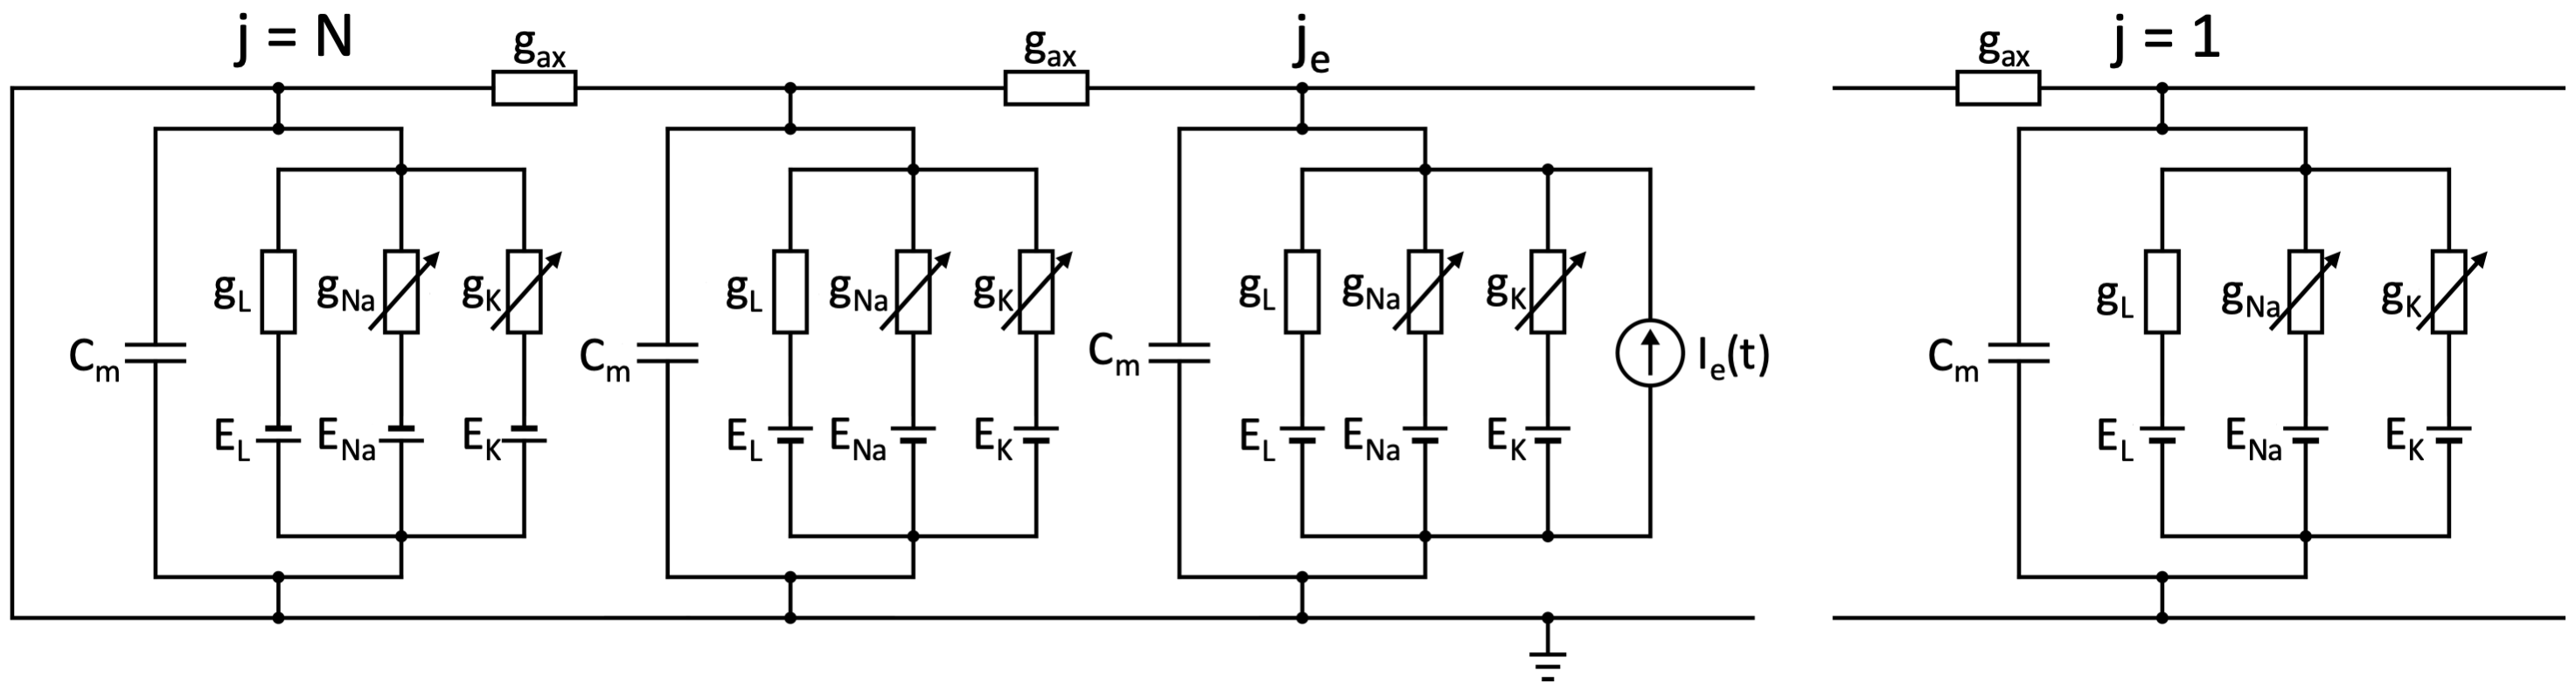
\includegraphics[width=1\textwidth]{Circuit_final.png}
        \caption{Circuit diagram of a multi-compartment Hodgkin-Huxley model. Compartment 1 is terminated as a 'sealed end' and 
        compartment N is terminated as a 'killed end'. Note that the connection between compartment 1 and compartment $j_{e}$ is not 
        shown for simplicity.}
    \end{figure}
    \newline The approximated DEQ for voltage response of compartment $j$ into which current is injected looks as shown below
    \begin{align*}
        V'_{j}(t + \Delta t) = V'_{j}(t) + \frac{\Delta t}{C_{m}}\left(I_{e}(t) \right. &+ g_{L}\left(E_{L}-V'_{j}(t)\right) + \bar{g}_{Na}m^{3}_{j}(t)h_{j}(t)\left(E_{Na}-V'_{j}(t)\right)\\
                                                                                        &+ \bar{g}_{K}n^{4}_{j}(t)\left(E_{K}-V'_{j}(t)\right) + g_{ax}\left(V'_{j-1}(t)-V'_{j}(t)\right)\\
                                                                                        &+ g_{ax} \left. \left(V'_{j+1}(t)-V'_{j}(t)\right)\right)
    \end{align*}
    Following Homework 4, voltage response for compartment $i$ where $0 < i < j$ is
    \begin{align*}
        V'_{i}(t + \Delta t) = V'_{i}(t) + \frac{\Delta t}{C_{m}}\left(\right. & g_{L}\left(E_{L}-V'_{i}(t)\right) + \bar{g}_{Na}m^{3}_{i}(t)h_{i}(t)\left(E_{Na}-V'_{i}(t)\right)\\
                                                                                        &+ \bar{g}_{K}n^{4}_{i}(t)\left(E_{K}-V'_{i}(t)\right) + g_{ax}\left(V'_{i-1}(t)-V'_{i}(t)\right)\\
                                                                                        &+ g_{ax} \left. \left(V'_{i+1}(t)-V'_{i}(t)\right)\right)
    \end{align*}
    As for compartment $i$ where $j < i < N$, we have
    \begin{align*}
        V'_{i}(t + \Delta t) = V'_{i}(t) + \frac{\Delta t}{C_{m}}\left(\right. & g_{L}\left(E_{L}-V'_{i}(t)\right) + \bar{g}_{Na}m^{3}_{i}(t)h_{i}(t)\left(E_{Na}-V'_{i}(t)\right)\\
                                                                                        &+ \bar{g}_{K}n^{4}_{i}(t)\left(E_{K}-V'_{i}(t)\right) + g_{ax}\left(V'_{i+1}(t)-V'_{i}(t)\right)\\
                                                                                        &+ g_{ax} \left. \left(V'_{i-1}(t)-V'_{i}(t)\right)\right)
    \end{align*}
    As regards the termini, membrane potential for compartment $j=N$ is set to 0 and for compartment $j=1$ we assume no axial current flowing out, and hence all membrane potential difference is due to 
    current flowing through the membrane
    \begin{align*}
        V'_{1}(t + \Delta t) = V'_{1}(t) + \frac{\Delta t}{C_{m}}\left(\right. g_{ax}\left(V'_{2}(t)-V'_{1}(t)\right) &+ g_{L}\left(E_{L}-V'_{1}(t)\right) + \bar{g}_{Na}m^{3}_{1}(t)h_{1}(t)\left(E_{Na}-V'_{1}(t)\right)\\
                                                                                        &+ \bar{g}_{K}n^{4}_{1}(t)\left(E_{K}-V'_{1}(t)\right)
    \end{align*}
    For the approximations of $m, h, n$ gating variables please refer to Homework 4.
\end{enumerate}
\end{document}
